\DiaryEntry{Numerical Linear Algebra, SVD}{2019-10-09}{Linear Algebra}

The \emph{reduced SVD} decomposes a matrix into three matrices as follows,

\bee
\Abf = \hat\Ubf \hat\Sigmabf \Vbf^H
\eee

where $\hat\Ubf$ is an $m \times m$ matrix with orthonormal columns, $\Sigmabf$ is an $n \times n$ diagonal matrix containing the singular values (these are positive real numbers) $\sigma_i$, and $\Vbf$ is an $n \times n$ martix with orthonormal columns. The column vectors in $\Ubf$ are the \emph{left singular vectors} whereas the column vectors in $\Vbf$ are the \emph{right singular vectors}.

A matrix-vector multiplication $\Abf \xbf$ can be interpreted as follows: First the vecotr $\xbf$ is expressed  as linear combination of the basis spanned by the columns of $\Vbf$. Then each direction in this new basis is scaled by the singular values $\sigma_i$. Finally, the result is used as components in a linear combination of the column vectors of $\hat\Ubf$.

The Figure below shows the size of the matrices involved.

\begin{figure}[hbt!]
\centering
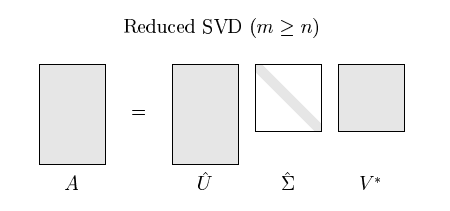
\includegraphics[scale=0.5]{images/num_lin_algebra_03_1.png}
\end{figure}

In the reduced SVD, the $n$ columns of the matrix $\Ubf$ are orthonormal vectors in an $m$-dimensional space $\mR^m$. Unless $m = n$, these vectors do not form a basis for $\mR^m$ (it's not enough vectors) and therefore $\hat\Ubf$ is not a unitary matrix.

If we extend the matrix $\hat\Ubf$ by $m-n$ additional orthonormal columns to obtain $\Ubf$, the columns of $\Ubf$ form a basis and $\Ubf$ is a unitary matrix. In order for the product to stay the same, we need to modify $\hat\Sigmabf$ as well; we need to ``zero-out'' the additionally introduced columns. So $\hat\Sigmabf$ is augmented at the bottom with $m-n$ rows of zeros; the resulting matrix $\Sigmabf$ has then size $m \times n$.


\begin{figure}[hbt!]
\centering
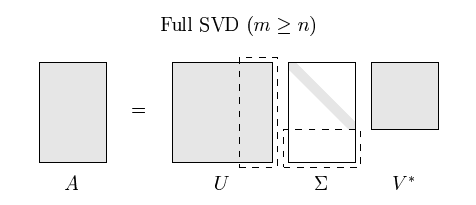
\includegraphics[scale=0.5]{images/num_lin_algebra_03_2.png}
\end{figure}

\paragraph{Example.} As an example, consider the following matrix

\bee
\Abf = \begin{pmatrix} 1& 3 \\ -1 & 5 \\ 8 & 2 \end{pmatrix}
\eee

Using this matrix in Julia for calculating the reduced SVD

\begin{verbatim}
using LinearAlgebra

A = [1 3; -1 5; 8 2]
r = svd(A)

r.U
3×2 Array{Float64,2}:
 -0.244521  -0.420991
 -0.116781  -0.881487
 -0.962586   0.213885

r.S
2-element Array{Float64,1}:
 8.473428460382687
 5.674593388673472

r.V
2×2 Adjoint{Float64,Array{Float64,2}}:
 -0.92388    0.382683
 -0.382683  -0.92388 

r.U*Diagonal(r.S)*r.V'
3×2 Array{Float64,2}:
  1.0  3.0
 -1.0  5.0
  8.0  2.0

r.U*r.U'
3×3 Array{Float64,2}:
 0.237024   0.399654    0.145329 
 0.399654   0.790657   -0.0761246
 0.145329  -0.0761246   0.972318

\end{verbatim}

Calculating the full SVD yields

\begin{verbatim}

rfull = svd(A, full=true)

rfull.U
3×3 Array{Float64,2}:
 -0.244521  -0.420991  -0.873485
 -0.116781  -0.881487   0.45754 
 -0.962586   0.213885   0.166378

rfull.S
2-element Array{Float64,1}:
 8.473428460382687
 5.674593388673472

rfull.V
2×2 Adjoint{Float64,Array{Float64,2}}:
 -0.92388    0.382683
 -0.382683  -0.92388 

rfull.U*[Diagonal(rfull.S) ;0 0]*rfull.V'
3×2 Array{Float64,2}:
  1.0  3.0
 -1.0  5.0
  8.0  2.0

rfull.U*rfull.U'
3×3 Array{Float64,2}:
 1.0           1.66533e-16   3.60822e-16
 1.66533e-16   1.0          -1.38778e-17
 3.60822e-16  -1.38778e-17   1.0 

\end{verbatim}

Here the reconstruction of $\Abf$ is a bit messy as we need to extend $\hat\Sigmabf$ to $\Sigmabf$ by inserting a zero-row at the bottom.

\subsection{SVD vs Eigenvalue Decomposition}

The eigenvalue decomposition is defined for non-defective, square matrices; we have

\bee
\Abf = \Xbf \Dbf \Xbf^{-1}
\eee

where $\Dbf$ is a diagonal matrix holding the eigenvalues and $\Xbf$ the linearly independent eigenvectors of $\Abf$.

The SVD uses two different bases (left and right singaulr vectors) , whereas the eigenvalue decomposition uses only one basis (column vectors in $\Xbf$). In addition, the two bases in the SVD are orthonormal whereas the eigenvalue decomposition uses a basis that is not orthonormal but ``only'' linearly independent. Finally, the SVD exists for all matrices (also non-square ones), whereas the eigenvalue decomposition need not even exist.

\subsection{Matrix Properties via SVD}

Many matrix properties can be deduced from the SVD. In the following, let $\Abf$ be a $m \times n$ matrix, $p = \min m,n$, and let $r \leq p$ denote the number of non-zero singular values of $\Abf$.

\begin{theorem} The rank of $\Abf$ is $r$, the number of non-zero singular values. \end{theorem}

\begin{theorem} The range of $\Abf$ is the vector space spanned by the column vectors $\ubf_1 \cdots \ubf_r$. The nullspace of $\Abf$ is the vector space spanned by the column vectors $\vbf_{r+1} \cdots \vbf_n$. \end{theorem}

\begin{theorem} $|| \Abf ||_2 = \sigma_1$ and $|| \Abf ||_F = \sqrt{\sigma_1^2 + \cdots \sigma_r^2}$. \end{theorem}

\begin{theorem} The non-zero singular values of $\Abf$ are the square roots of the non-zero eigenvalues of $\Abf^T \Abf$ or $\Abf \Abf^T$.\end{theorem}

We have

\bee
\Abf \Abf^T = (\Ubf \Sigmabf \Vbf) (\Ubf \Sigmabf \Vbf)^T = \Ubf \Sigmabf \Vbf \Vbf^T \Sigmabf \Ubf^T = \Ubf (\Sigmabf \Sigmabf) \Ubf
\eee

\begin{theorem} If $\Abf = \Abf^T$, then the singular values of $\Abf$ are the absolue values of the eigenvalues of $\Abf$. \end{theorem}

\begin{theorem} The determinant if $\Abf$ equals the product of its singular values, $\det \Abf = \prod_i \sigma_i$. \end{theorem}

We have

\bee
\det \Abf = \det (\hat \Ubf \hat\Sigmabf \Vbf^H) = \det \hat\Ubf \det \hat\Sigmabf \det \Vbf^H = \prod_i \sigma_i
\eee

because the determinant of a matrix product equals the product of the factor determinants and the determinant of an orthonormal matrix is one.


\subsection{Low-rank Approximations}

We can gain further insight into the SVD by rewriting the matrix $\Abf$ as follows

\bee
\Abf = \sum_{j=1}^r \sigma_j \ubf_j \vbf_j^H
\eee

This gives the interpretation of $\Abf$ as a sum of rank-one matrices. These rank-ones matrices are special in the sense as the partial sum is the optimal approximation of $\Abf$. Define

\bee
\Abf_\nu = \sum_{j=1}^\nu \sigma_j \ubf_j \vbf_j^H
\eee

and then we have

\bee
|| \Abf - \Abf_\nu ||_2 = \sigma_{\nu+1} \quad \text{and} \quad || \Abf - \Abf_\nu ||_F = \sqrt{\sigma_{\nu+1}^2 + \sigma_{\nu+2}^2 + \cdots + \sigma_{r}^2}
\eee



%%% Local Variables:
%%% mode: latex
%%% TeX-master: "journal"
%%% End:
